\documentclass{eceasst}
% This is the source of the author documentation
% for the ECEASST document class.

% Required packages
% =================
\usepackage{subfig}

% Volume frontmatter
% ==================
% Volume frontmatter for OCL 2011
% =====================================
\volume{44}{2011} % Volume number and year
\volumetitle{% Title of the volume (optional)
Proceedings of the\\
Workshop on OCL and Textual Modelling\\
(OCL 2011)}
\volumeshort{% Short title of the volume (optional)
Proc.\ OCL 2011}
\guesteds{% Multiple guest editors
Jordi Cabot, Tony Clark, Manuel Clavel, Martin Gogolla}


% Article frontmatter
% ===================
\title{% Title of the article
Modeling the OCL Standard Library}
%\short{% Short title of the article (optional)
%Modeling the OCL Standard Library}
\author{% Authors and references to addresses
Edward Willink\autref{1}}
\institute{% Institutes with labels
\autlabel{1} \email{ed \_at\_ willink.me.uk}, \url{http://www.eclipse.org/modeling}\\
Eclipse Modeling Project}

\abstract{
OCL is widely used by UML and other languages to constrain meta-models and perform evaluations on models. The OCL specification is the result of diligent but time-constrained human endeavor and so contains many inconsistencies, most of which are relatively easy to ignore as obvious typographical mistakes. However the need to ignore minor discrepancies undermines rigorous treatment of more significant issues. The minor issues can be substantially eliminated by auto-generating the specification. This paper provides early community visibility of proposed solutions to a variety of issues that arose while developing a model for the OCL Standard Library that forms the core of the OCL specification.}
\keywords{OCL, meta-model, library, auto-generation, templates}

\begin{document}
\maketitle
\section{Introduction}

The Object Constraint Language (OCL) evolved, initially within the Unified Modeling Language (UML). As part of the UML 2.0\cite{UML-2.0} revision activities, OCL was separated out as a separate specification in recognition of OCL's utility in non-UML contexts. Unfortunately the UML Revision Task Force had insufficient resources to complete the revision of OCL 1.6\cite{OCL-1.6} to align with UML 2.0. A partially revised OCL 2.0 draft\cite{OCL-2.0-draft} was all that was available to accompany UML 2.0.

When the QVT specification was developed, the utility of OCL was recognized and OCL 2.0\cite{OCL-2.0} formed the basis for QVT 1.0\cite{QVT-1.0}. The QVT Finalization Task Force also finalized the OCL 2.0 specification, but had insufficient resources to perform the very detailed proof reading and consistency checking for a specification involving so many cross-references.

The OCL 2.2\cite{OCL-2.2} revision addressed a relatively small proportion of the outstanding issues.

The OCL 2.3\cite{OCL-2.3} revision addressed a substantial inconsistency that arose when an undefined value evolved to a \verb|null| or \verb|invalid| value and a major under-specification of the concrete syntaxes of terminals. However the bulk of the inconsistencies remained.

\subsection{Revision}

The Object Management Group revision process for these specifications starts when an issue is raised against a specification; anyone can raise an issue. Each issue should be addressed by a Revision Task Force leading to a No-Change, Duplicate, Merged or Resolved response. In practice many issues have been Deferred through lack of time. Each issue that requires a change requires a written proposal to be prepared in which the issue is discussed and the associated editorial changes are clearly identified. Proposals are voted on by the Revision Task Force and in due course a revised specification is prepared, approved by the Architecture Board and ultimately adopted by the OMG.

An attempt was made to pursue this process to resolve the incomplete change in alignment between UML 1.x's AssociationEnd and UML 2.x's Property class. The detailed changes proved too laborious. Now that good modeling technology tools are readily available, it is an anachronism that the OCL specification that underpins so many of the tools is maintained manually.

It was therefore decided to exploit models to capture as much of the specification as practical and then to auto-generate the specification from the models. Auto-generation should then ensure that typographic errors in technical content are almost non-existent, and should enable the detailed lists of editorial changes required by the OMG process to be auto-generated as well.

\subsection{Models}

The Essential OCL can be modeled using 5 models:
\begin{itemize}
\item the UML meta-model (UML Infrastructure)
\item an OCL Standard Library Model (OCL Clause 11)
\item an Abstract Syntax Meta-Model (OCL Clause 8)
\item a Concrete Syntax to Abstract Syntax Mapping (OCL Clause 9)
\item a Run-time Semantics Model (OCL Clause 10)
\end{itemize}

Complete OCL requires similar smaller models to flesh out Clause 12.

The models above are interdependent, with UML heavily reliant on OCL expressions, whose operators are defined by the OCL Standard Library. The OCL Standard Library has limited dependencies on the Abstract Syntax and Run-time Semantics, so defining the OCL Standard Library and consequently expression validity is the key to modeling the whole OCL specification.

Each version of an OCL 2.x specification states, in its Scope statement, that it is aligned with a corresponding UML 2.x specification. Sadly this statement is only an aspiration at present. Nonetheless we must proceed towards that goal and so clearly an OCL Standard Library Model should be describable by UML.

\subsection{Paper}

In this paper we discuss many of the issues that have arisen in building a UML-aligned meta-model for the OCL Standard Library and using that meta-model to define the Library. In a companion paper\cite{OCL-UML} we discuss issues arising from attempting to achieve UML-alignment more generally and establish the meaning of an OCL model as a combined instance of the merged UML and OCL meta-models.

It is hoped that by presenting the community with an early insight into changes that may be proposed for OCL 2.4, the community may be able to contribute constructively before, rather than after, the revised specification is adopted.

A prototype of the modeled OCL Standard Library may be found in the optional Examples and Editors of the Indigo release of Eclipse OCL\cite{MDT/OCL}, which is officially released in June 2011 and for which milestone builds have been available since December 2010. The prototype defines a Domain Specific Language to specify the OCL Standard Library, and uses Xtext\cite{TMF/Xtext} tooling to provide a rich editing capability for the DSL. This facilitates entry of OCL postconditions on library operations and validates that these postconditions are consistent with the library model.

The clarifications outlined below involve very few if any, actual changes to the user perception of OCL; they merely enable the specification to say what many users think it already says. Of course OCL implementations that have resolved ambiguities in alternative directions may see a change. However even changes in the specification need not impact compatibility, since with substantial parts of the OCL semantics migrating to the library model, it may be possible to encapsulate the semantics of a particular OCL tool version in a corresponding OCL Standard Library model and so preserve precisely those semantics for those users that require them.

In Section \ref{LibraryUtility} we discuss the basic properties of a library model, then in Section \ref{LibraryModel} we show how a variety of OCL concepts can be captured by the library model. With a modeling capability established, in Section \ref{LibraryContent} we identify aspects of the library that deserve revision and in Section \ref{AwkwardOperations} we examine a number of operations that are difficult to model. Further minor revisions to enhance modeling are considered in Section \ref{FurtherModeling}. Finally we conclude. 

\section{Library Utility}\label{LibraryUtility}

We start by identifying ways in which an OCL model of the OCL Standard Library can be useful.
 
\subsection{Consumable}

While auto-generation of the OCL specification may be a primary motivation for modeling the OCL Standard Library, provision of a consumable machine readable model is equally valuable. It avoids the need for OCL implementors to transcribe the specification, avoids associated transcription errors, and so avoids inconsistencies between alternate implementations. Availability of a model should encourage tools to use declarations in the model rather than hand coding to realize important tooling behaviors.

Definition of the library requires concepts that cannot be expressed in Essential OCL or Complete OCL, and so a Domain Specific Language with a new Concrete Syntax is used to define library elements. A simple example of part of the \verb|Integer| definition is shown in Figure~\ref{fig:SimpleExample}.

\begin{figure}
  \begin{center}
    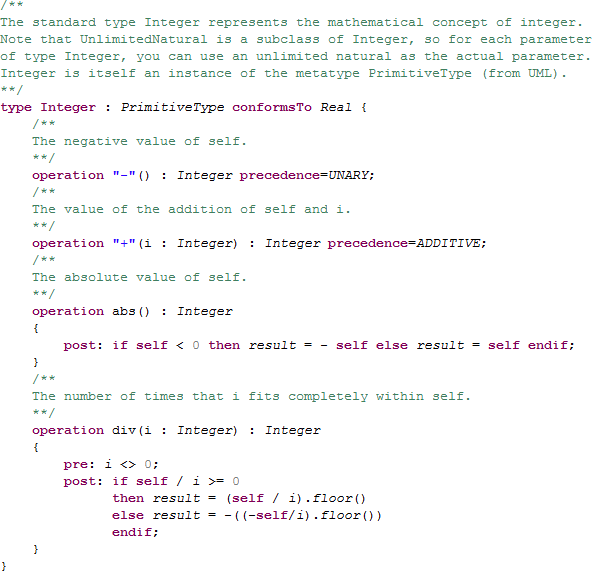
\includegraphics[width=5.75in]{SimpleExample.png}
  \end{center}
  \caption{Simple Library Concrete Syntax Example.}
  \label{fig:SimpleExample}
\end{figure}

The \verb|Integer| type is defined to conform to the \verb|Real| type and to be an instance of the \verb|PrimitiveType| meta-type.

Four operations are defined, the first with a precedence labeled as \verb|UNARY|, and the second with a precedence labeled as \verb|ADDITIVE|. Precedence is discussed in Section \ref{Precedence}.

The first operation is unary minus. It takes no arguments and returns an Integer. It has a precedence and so may be used as a prefix operator.

The second operation is binary plus. It takes an Integer argument and returns an Integer. It has a precedence and so may be used as an infix operator.

The third and fourth operations have simple names that do not require quotes; they have associated preconditions and postconditions expressed in OCL. These are verified by the editor tooling.

When applied to \verb|OrderedSet::indexOf|, the typo involving \verb|i| rather than \verb|result| is detected as shown in Figure~\ref{fig:OrderedSet_indexOf}.

\begin{figure}
  \begin{center}
    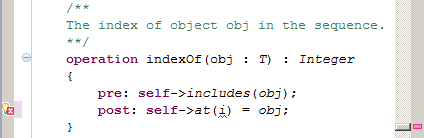
\includegraphics[width=4.1in]{OrderedSet_indexOf.png}
  \end{center}
  \caption{OrderedSet::indexOf with error.}
  \label{fig:OrderedSet_indexOf}
\end{figure}

\subsection{Implementable}

If the OCL Standard Library is to be used by practical OCL tools, the library model must provide a body for every operation and iteration. This is difficult for the simplest operations whose body is just `obvious' and potentially inefficient for more complicated bodies. OCL tools may wish to provide their own more optimum implementation. The DSL therefore allows an arbitrary string to be specified for use by the tooling. The usage for Eclipse OCL is shown in Figure~\ref{fig:ImplementationExample}. The string identifies the Java class that realizes the defined library feature.

\begin{figure}
  \begin{center}
    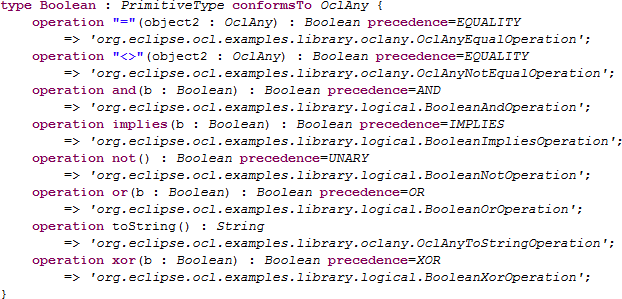
\includegraphics[width=5.75in]{ImplementationExample.png}
  \end{center}
  \caption{ImplementationExample.}
  \label{fig:ImplementationExample}
\end{figure}

A practical tool-independent OMG distribution might facilitate a simple automated conversion to tool-specific form by providing unique strings such as \verb|org.omg.ocl.lib.Boolean.xor|.

\subsection{Auto-generation}

In order to support full specification auto-generation, all editorial content must be present in the model. Simplistically, this can be provided by embedding description in preceding comments, as in Figure~\ref{fig:SimpleExample}. Providing sufficient richness to capture the limited usage of italics, bullets and figures currently in the specification is work in progress. A very limited subset of HTML markup is probably the solution since the Xtext tooling already supports embedded HTML.

Once the full description is present in the model, implementations may present the description to users in their documentation, help or hover text. Acceleo\cite{M2T/Acceleo}, which is the Eclipse implementation of the OMG MOFM2T\cite{MOFM2T} model-to-text transformation language, is being used to auto-generate Clause 11, the OCL Standard Library, from its OCL model.

\subsection{Extensible}

The term OCL Standard Library is something of a misnomer since the library has evolved incompatibly between OCL 2.x releases, and since it is extended by both QVT Operational and MOFM2T.

It is highly desirable to allow users or third parties to provide extended, alternate or additional libraries and so foster a growing collaborative community.

The library syntax therefore supports an import statement to allow a library to extend or exploit other libraries. Packages, types and features with identical hierarchical names (including parameter types for operations) are merged, provided no conflicts arise. This allows addition but not removal of

\begin{itemize}
\item packages and types to packages
\item features, invariants and conformances to types
\item preconditions, postconditions, bodies and implementations to operations or iterations
\item initializations and derivations to properties
\end{itemize}

The merge uses the same yet-to-be-defined merge semantics as for Complete OCL.

\section{Library Model}\label{LibraryModel}

The UML-aligned OCL pivot meta-model is discussed in the companion paper\cite{OCL-UML}. In this section we examine library concepts that require modeling, but for which there is either no UML or OCL representation, or for which the prevailing OCL representation is inconsistent with UML.

\subsection{Precedence and Associativity}\label{Precedence}

The precedence of \verb|and|, \verb|or| and \verb|xor| was changed in the OCL 2.2 specification, so it is desirable to model precedence in order to allow either OCL 2.0 or 2.2 semantics to be used simply by selecting a corresponding OCL Standard Library Model. It is also desirable to allow languages that extend OCL freedom to redefine precedence and associativity to whatever is appropriate for the extended language.

Provision of a precedence label, as in Figure~\ref{fig:SimpleExample}, specifies that a no argument operation can also be used as a prefix operator, and that a single argument operation can be used as an infix operator. Operators sharing a precedence label are equi-precedence, and precedences are ordered by a separate precedence ordering statement as shown in Figure~\ref{fig:Precedence}. In the OCL 2.2 example, \verb|AND| has higher precedence that \verb|OR| so the expression \verb|a and b or c and d| should be interpreted as \verb|(a and b) or (c and d)|. Precedences orderings may be extended by merging non-conflicting orderings from imported libraries.

\begin{figure}
  \begin{center}
    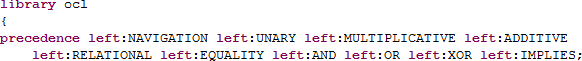
\includegraphics[width=5.75in]{Precedence.png}
  \end{center}
  \caption{Precedence Ordering.}
  \label{fig:Precedence}
\end{figure}

All operators are left associative in OCL, that is \verb|a.b.c| is \verb|(a.b).c| rather than \verb|a.(b.c)|. The modeling allows right associativity to be specified.

\subsection{Conformance}

The conformance of Collection upon OclAny was changed in the OCL 2.2 specification, so this too should be model-able.

The \verb|conformsTo| declaration in Figure~\ref{fig:SimpleExample} is similar to an \verb|extends| or \verb|implements| in Java; it may specify a comma-separated list of types to which a type conforms.

With conformance defined in the model, many conformance statements throughout the OCL specification can be eliminated as well as some definitions of a \verb|conformsTo()| helper operation.

Much of the conformsTo relationship can be captured structurally, if OCL tooling loading a UML meta-model creates a conformsTo relationship for each generalisation relationship and adds a conformsTo Classifier relationship for every root class. However operational conformance is still needed to define:

\begin{itemize}
\item OclVoid conforms to all types (except OclInvalid).
\item Collection conformance requires conformance of collection and element types.
\item Tuple conformance requires part name match and type conformance.
\end{itemize}

\subsection{Templates or Generics}

UML defines templates which are necessary to define
\begin{itemize}
\item Collections as classes with a single template parameter
\item Tuples which have many named template parameters
\item the Collection::product operation which has an operation template parameter
\end{itemize}

Figure~\ref{fig:TemplateExample} shows an example type template.

\begin{figure}
  \begin{center}
    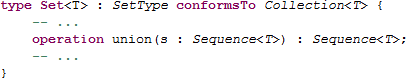
\includegraphics[width=4.0in]{TemplateExample.png}
  \end{center}
  \caption{Template Concrete Syntax Example.}
  \label{fig:TemplateExample}
\end{figure}

Note that this use of templates for library definition purposes does not require OCL to support templates; it is full alignment of OCL with UML that requires it.

The usage of \verb|< >| for templates is well-established in many languages such as C++, Java and even UML. Unfortunately OCL currently uses \verb|( )| to parameterize its Collection and Tuple types. This suggests that introduction of templates into OCL should use \verb|( )| for compatibility.

Eclipse OCL has successfully used \verb|( )| for templates in prototype tooling. Usage of this tooling indicates that \verb|( )| are acceptable but a little disconcerting for type templates. But for operation templates \verb|( )| are very confusing since an operation name may then be followed by one or two parenthesized clauses. The last clause is always for operation arguments or parameters. The first clause is optional and provides the template parameters or bindings. Eclipse OCL prototype tooling has therefore switched to using \verb|< >|. Compatibility is preserved by allowing \verb|( )| following an explicit Collection name or the Tuple keyword.

It therefore seems appropriate for introduction of template functionality to OCL to align with UML and to use \verb|< >|. The existing usage of \verb|( )| can be deprecated. \verb|< >| are used throughout this paper, except where the template clause is obvious and can be omitted for clarity.  

\subsection{Collection::product(...)}

Examination of the collection product operation reveals that it uses both type and operation template parameters. These are defined as shown in Figure~\ref{fig:TemplateOperation}.

\begin{figure}
  \begin{center}
    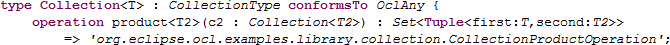
\includegraphics[width=5.75in]{TemplateOperation.png}
  \end{center}
  \caption{Template Operation Concrete Syntax Example.}
  \label{fig:TemplateOperation}
\end{figure}

The return type demonstrates the construction of a Set of Tuples whose element types are defined by the type template parameter T and the operation template parameter T2.

This provides an explicit declaration for T and T2, which are currently left to the reader's intuition.

\subsection{Iterators and Iterate}

\begin{figure}
  \begin{center}
    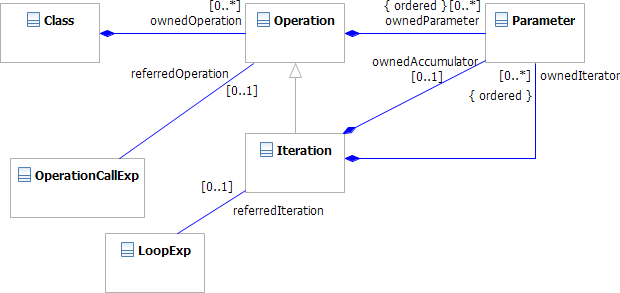
\includegraphics[width=5.75in]{Iteration.png}
  \end{center}
  \caption{Iteration and LoopExp.referredIteration.}
  \label{fig:Iteration}
\end{figure}

UML defines an Operation and associated Parameters. An iterator operation is similar to an operation but it also has Iterators, and the \verb|iterate| operation has an Accumulator as well. Some form of UML extension is required to model iterator operations. Extending Parameter kinds from  IN, INOUT, OUT and RESULT to accommodate ITERATOR and ACCUMULATOR was considered but found to be unhelpful in the context of references from OperationCallExp and LoopExp.

An Iteration class is therefore introduced, as shown in Figure~\ref{fig:Iteration}. Iteration extends Operation with additional ownedIterator and ownedAccumulator properties; the ownedParameter is re-used for the iteration body\footnote{This is semantically consistent; a parameter is externally bound. However re-using ownedParameter for iterators and then introducing ownedBody rather than ownedIterator would be slightly simpler.}. As an extension of Operation, iterations may be contained by the ownedOperation feature of a Class and so require no further changes. Introduction of a LoopExp::referredIteration analogous to OperationCallExp::referredOperation eliminates the need for iterations to be accessed by a vague name lookup at run-time.

Figure~\ref{fig:IterationExample} shows that iterate and iterator operations can be defined in a very similar fashion to operations, re-using the semi-colon and vertical bar from the iteration call concrete syntax. 

Iterations taking variable numbers of iterators are separately declared for each alternative.

\subsection{Lambda Expressions}

\begin{figure}
  \begin{center}
    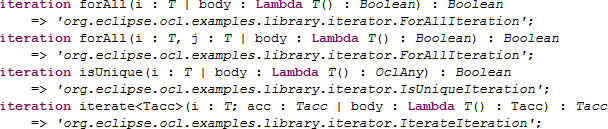
\includegraphics[width=5.75in]{IterationExample.png}
  \end{center}
  \caption{Iteration Concrete Syntax Example.}
  \label{fig:IterationExample}
\end{figure}

The equivalent iterator operation declarations to those in Figure~\ref{fig:IterationExample} in the OCL specification variously omit the final body argument or resort to textual substitution of the italicized body expression within the iterator exposition. The required type signature is defined by commentary and sometimes well-formedness rules. On closer examination the body expression is clearly an implicit form of a Lambda Expression.

Following a casual query at the OCL Workshop in 2010, as to whether OCL should support Lambda Expressions, a discussion on the LinkedIn OCL Users Group\cite{LinkedIn} generally welcomed their introduction. The declarations in Figure~\ref{fig:IterationExample} therefore use a Lambda Type to specify the constraints on the body expression. The syntax of a Lambda type draws on the Tuple and Operation signatures.

\verb|Lambda| context-type \verb|(| parameter-type-list \verb|) : | context-type

An ExpressionInOcl is also similar to a Lambda Expression but there is one important difference. An ExpressionInOcl is self-contained with all variable references terminated by context, parameter or result variables. An Iteration body has access to the invoking environment, so the analysis resolves variable references, some of which may be implicit, to the appropriate variables which are then available for access while the iteration is evaluated.

The signatures provided above use the iterator type as the lambda expression context-type.

\section{Library Content}\label{LibraryContent}

Once an ability to define an OCL Library has been established, some problems with the content of the OCL Standard Library arise and can be addressed. 

\subsection{Covariant Operation Overloading}

OCL specifies that OCL is aligned with UML, and UML specifies that the semantics of operation overloading is an implementation variation point. This unfortunately means that the utility of all overloaded operations is unclear in both OCL and UML. OCL must therefore define an operation overloading semantics. After discussion with a variety of concerned parties, invariant overloading semantics like Java seems appropriate. In Java, all overloads of \verb|Object.equals(Object)| must have an Object argument.

For OCL, the most derived unique compatible operation signature can be statically determined when the OCL expression is parsed and persisted as the target of an OperationCallExp::referredOperation in the AST. When evaluated, the dynamic type of the expression source can be used to select the most derived visible operation with the same signature. Analysis of UML 2.4, identified a couple of places where covariant overloading had been assumed; these usages were not significant and await correction in UML 2.5.

Covariant overloading allows a derived operation argument type to vary with the derived source type. This practice is widespread in the OCL standard library, where the equality operation \verb| OclAny::=(OclAny)| is overloaded by \verb|Collection::=(Collection)|.

If evaluation complexity is to be avoided, the library must be revised to eliminate covariant overloading.

\subsection{Collection Hierarchy}

The OCL 2.3 Collection hierarchy and conformance is shown in Figure~\ref{fig:Collections_2_2}\footnote{using $< >$ rather than a UML template to avoid tooling limitations}.

\begin{figure}
  \begin{center}
    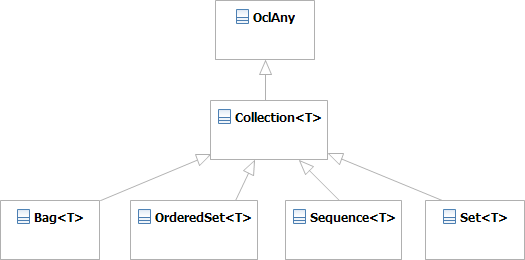
\includegraphics[width=5.0in]{Collections_2_2.png}
  \end{center}
  \caption{OCL 2.3 Collection Hierarchy.}
  \label{fig:Collections_2_2}
\end{figure}

There is limited declaration sharing between the Collection kinds and so when OrderedSet was introduced, it appears that its definition was cut and paste from Sequence. Unfortunately not all operations were reviewed to accommodate uniqueness of content, and insufficient Set operations were added. 

These problems are discussed by B\"{u}ttner\cite{Buttner} who observes that Set is-a Bag and OrderedSet is-a Sequence and so proposes the refactoring shown in Figure~\ref{fig:Collections_Buettner}.

\begin{figure}
  \begin{center}
    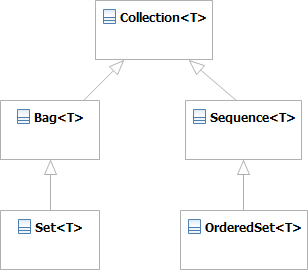
\includegraphics[width=3.0in]{Collections_Buettner.png}
  \end{center}
  \caption{Collection Refactoring proposed by Buettner.}
  \label{fig:Collections_Buettner}
\end{figure}

This refactoring eliminates some duplication and inconsistency. For instance, \verb|Set::asBag()| is doubly redundant;  it can now be inherited, and the associated kind conversion is no longer needed.

Further redundancy arises once covariant overloads are removed. The OCL 2.3 specification defines each of:

\verb|Bag::union(Bag<T>):Bag<T>|,

\verb|Bag::union(Set<T>):Bag<T>|,

\verb|Set::union(Bag<T>):Bag<T>|,

\verb|Set::union(Set<T>):Set<T>|.

With the refactored hierarchy, the mixed Set/Bag signatures are redundant since Set conforms to Bag. We need only:

\verb|Bag<T>::union(Bag<T>):Bag<T>|

\verb|Set<T>::union(Set<T>):Set<T>|

Introduction of a further UniqueCollection as shown in Figure~\ref{fig:Collections_2_4} provides further opportunities to eliminate redundant declarations.

\begin{figure}
  \begin{center}
    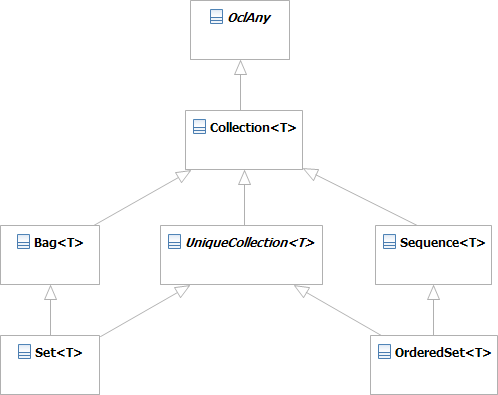
\includegraphics[width=4.5in]{Collections_2_4.png}
  \end{center}
  \caption{Further Collection Refactoring.}
  \label{fig:Collections_2_4}
\end{figure}

The Set operations that are also applicable to OrderedSet may be placed in UniqueCollection so that Set and OrderedSet have consistent functionality. For instance \verb|Set::-(Set):Set| may be moved to \verb|UniqueCollection::-(UniqueCollection):Set|. This will avoid the need to convert OrderedSet to a Set in order to use a variety of Set operations.

\subsection{Collection Operation Arguments}

The current specification of a library operation such as \verb|Bag::excluding(object : T)| leaves the semantics of \verb|T| unclear. Is \verb|T| the same or another type to the collection element type \verb|Bag<T>|? Clause 11.6 has a preamble defining \verb|T|, but does this apply to Clause 11.7 too?

A Java programmer will be surprised if the behavior does not support error-free `removal' of inappropriate objects in the same way as \verb|Collection<T>.remove(Object)|.

A user expecting very strong type checking may be disturbed if inappropriate types are silently ignored.

A modeled library requires the specification to explicitly choose between:

\verb|Bag<T1>::excluding(object : T1)|

\verb|Bag<T1>::excluding(object : OclAny)|

\verb|Bag<T1>::excluding<T2>(object : T2)|

When dealing with \verb|null| collection content, OCL provides a safe silent helpful behavior, so allowing the \verb|excluding| operation to ignore inappropriate exclusions seems appropriate. This eliminates the first option. Introduction of the T2 template parameter is explicit but redundant so a Java-like \verb| Bag<T>::excluding(object : OclAny)| seems the better clarification.

\subsection{Modularity}

The OCL specification provides support for concepts that have very specialized UML utility. Given OCL's increasing use in non-UML applications, it seems appropriate to eliminate the specialized concepts from OCL and migrate their specification to the relevant UML packages. In exchange, OCL should support merging of modules that extend a core behavior\cite{Chimiak-Opaka}.

The import statement in the Library DSL supports migration of the OclMessage and associated declarations to perhaps UmlMessage.oclstdlib.

The UML package merge defining the OCL pivot meta-model\cite{OCL-UML} supports the merge of additional packages.

When Clause 9 has a complete exposition of the grammar for the concrete syntax, this too can support a merge of additional grammar constructs. 

The most obvious concepts for elimination are messages and states. It is unclear whether further modularization as suggested by Akehurst\cite{Akehurst} isolating tuples, iterators, collections and primitives is useful. Perhaps even finer grain modularization could be useful so that either Real or UnlimitedNatural could be omitted.

\section{Awkward Operations}\label{AwkwardOperations}

Most of the library is easy to model using the concepts outlined above. However a few operations are more troublesome.

\subsection{Implicit as-set: OclAny::oclAsSet()}

The OCL specification variously specifies that, for a defined object,  an \verb|->| operation implicitly creates either a set or a bag containing that object. If the object is null an empty bag or set is created. If the object is invalid, no collection created, rather the invalid value propagates. This creation has to occur at run-time since, unlike the equivalent implicit collect shorthand, there is no way to reify the set/bag creation at compile-time. It is necessary to know whether the object is null or invalid in order to synthesize creation of the appropriate CollectionLiteralExp content.

Introduction of an OclAny::oclAsSet() operation allows the analysis to be performed statically and persisted in the AST. The complexities of null and invalid can then be resolved by dynamic dispatch selecting between:

\verb|OclAny::oclAsSet()| -- returns \verb|Set{self}|

\verb|OclVoid::oclAsSet()| -- returns \verb|Set{}|

\verb|OclInvalid::oclAsSet()| -- returns \verb|invalid|

Alternate semantics may be configured by binding the OclAny and or derived operations to a different implementation.

The above declarations conveniently ignore the return type. Static type information is lost by a simple declaration such as \verb!OclAny::oclAsSet() : Set<OcAny>!. This is resolved by introducing  a reserved template parameter \verb!OclSelf! to capture the statically determined context type.

The declaration \verb!OclAny<OclSelf>::oclAsSet() : Set<OclSelf>! therefore allows \verb|'aString'->forAll(...)| to use \verb|Set<String>| as the context type and consequently \verb|String| rather than \verb|OclAny| as the iterator type.

\subsection{Reflection: OclAny::oclType()}

The oclType operation is irregular in that its return is an expression whose value is a type rather than an object. The operation return is therefore at a different meta-level.

This operation was not present until OCL 2.2, since \verb!Element::getMetaClass()! was  thought to support reflection. Unfortunately \verb!getMetaClass()! is defined by MOF which is not merged to form part of a UML meta-model.

In OCL 2.2, the specification is: \verb!OclAny::oclType() : Classifier! with Classifier confusingly playing a role at two different meta-levels, even though EMOF has no Classifier.

Examination of the postcondition for \verb|Sequence::first()| reveals a fully reflective usage of oclType to access the element type of the sequence:

\verb|if self.oclType().elementType.oclIsKindOf(CollectionType)|. 

The \verb|CollectionType::elementType| access requires oclType to return at least a CollectionType. An \verb|oclAsType(CollectionType)| cast could be introduced to fix the above example, but it demonstrates that the
derived type is statically determinate and that it is useful to make that type available.

\begin{figure}
  \begin{center}
    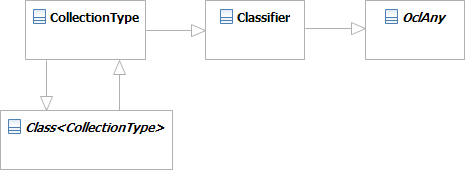
\includegraphics[width=4.5in]{Class.png}
  \end{center}
  \caption{Class Conformance Relationships.}
  \label{fig:Class}
\end{figure}

The templated Class type, shown in Figure~\ref{fig:Class}, provides \verb|Class<CollectionType>| as the meta-class of CollectionType. Both CollectionType and its meta-class conform to Classifier and OclAny since conformance of all types to OclAny occurs on  both the model and meta-model level. 

Use of the OclSelf template parameter in conjunction with the templated meta-class resolves the problem with the oclAsSet return type. A consistent specification is:

\verb!OclAny::oclType<OclSelf>() : Class<OclSelf>!

The \verb!Class<T>! is used to propagate static type information. \verb!Class<T>! conforms to Classifier so a fully reflective tower is possible and it is meaningful to write:

 \verb!self.oclType().oclType().oclType().ownedAttributes!

\subsection{Type-cast: OclAny::oclAsType(...)}

The oclAsType operation is similarly irregular in that its argument is an expression whose value is a type rather than an object. The operation argument is therefore at a different meta-level.

In OCL 1.6, this is specified as: \verb!OclAny::oclAsType(typename : OclType) : T!  with T ill defined and OclType a mysterious Enumeration over an open set of all possible classifiers.

In OCL 2.0, this is declared as: \verb!OclAny::oclAsType(typespec : OclType) : T! with OclType now a little-understood power-set.

In OCL 2.2, the declaration is: \verb!OclAny::oclAsType(type : Classifier) : T! with T still ill-defined and the use Classifier at a different meta-level is unexplained. The descriptive text refers to `t' rather than `type'.

In OCL 2.3, the declaration is unchanged but the typo in the descriptive text now refers to`T' rather than `type'.

The underlying rationale seems to be to try and establish an identity for a meta-type without imposing the cost of reflective tower that would arise with a true meta-type. This was not a requirement in the OCL 2.0 Request For Proposals\cite{OCL-RFP}, and the usage of oclType() requires reflection anyway, so it seems appropriate to provide reflection rather than an inconsistent facility that does not.

A consistent specification is: \verb!OclAny::oclAsType<T>(type : Class<T>) : T!

This exploits the conformance of \verb!T! to \verb!Class<T>! to preserve the static type. It assumes that the model of the unspecified TypeValue class is specified to be a \verb!Class<T>!. 

\subsection{OclAny::allInstances(...)}

The allInstances operation is irregular in that it is the only class operation; all other operations are instance operations. This prompted OMG Issue 8937\cite{OMG-Issue-8937} to suggest that `::' rather than `.' should be used when invoking allInstances in the concrete syntax. However allInstances is not a Classifier class operation, rather it is an operation on the statically determined derived Classifier class. Thus all instances of Person are returned by the invocation  \verb!Person.allInstances()! which is handled by the  \verb!Classifier::allInstances()! operation. There is no such operation as \verb!Person::allInstances()!. 

A consistent specification for this is:

\verb!static Classifier::allInstances<OclSelf>() : Set<OclSelf>!

Once again OclSelf solves the typing problem enabling the return type to use the statically determined derived Classifier type. The `static' keyword indicates that the source should be a type-valued expression. This ensures that  \verb!aPerson.allInstances()! can be diagnosed as an undefined operation.

\subsection{Collection::collect(...)}

The collect() iteration is potentially awkward since the return type is a flattened collection and consequently there is no unique mapping from input to output types. 

In OCL 2.0, it might appear that a \verb!Bag<T>! return value could have been produced by an input value corresponding to any of the \verb!Bag<T>!, \verb!Bag<Bag<T>>! or \verb!Bag<Bag<Bag<T>>>! types, but the first level element types have no mutual conformance so such content is a type error. OCL 2.0 does not support mixed depth collections.

In OCL 2.2, Collection conforms to OclAny, and so a collection may contain both collection and non-collection values. However,  for a heterogeneous collection, the existing type system cannot achieve greater precision than  \verb!Collection<OclAny>!, since OclAny is the only common type of a collection and a non-collection.

This lack of precision makes the declared return type of the collect operation and consequently an implicit collect almost unusable for heterogeneous collections. Fortunately this language limitation does not impact the collect() declaration and so  we only need declarations that are valid for homogeneous collections.

\begin{verbatim}
Collection<T>::collect<T2>(i : T |
  body : Lambda T(): T2) : Collection<T2>
Collection<T>::collect<T2>(i : T |
  body : Lambda T(): Collection<T2>) : Bag<T2>
Bag<T>::collect<T2>(i : T |
  body : Lambda T(): T2) : Bag<T2>
Sequence<T>::collect<T2>(i : T |
  body : Lambda T(): T2) : Sequence<T2>
Sequence<T>::collect<T2>(i : T |
  body : Lambda T(): Sequence<T2>) : Sequence<T2>
\end{verbatim}

Note that the final declaration for Sequence is not an overload. Introduction of modeled signatures highlights a gap in the specification as to what happens when unordered content is collected from an ordered collection. The lack of overload above gives an unambiguous interpretation; mixed ordering collect yields a Bag.

\section{Further Modeling}\label{FurtherModeling}

The preceding sections have identified ways in which awkward declarations can be modeled. We now examine ways in which some well-formedness rules can be modeled more overtly.

\subsection{Comparable}

The \verb|Collection::min| operation specifies ``Elements must be of a type supporting the min operation. The min operation - supported by the elements - must take one parameter of type T and be both associative and commutative. UnlimitedNatural, Integer and Real fulfill this condition.''

The \verb|sortedBy| iteration requires ``The type of the body expression must have the $<$ operation defined.''

\begin{figure}
  \begin{center}
    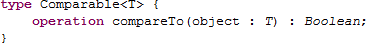
\includegraphics[width=4.0in]{Comparable.png}
  \end{center}
  \caption{Comparable.}
  \label{fig:Comparable}
\end{figure}

These similar functionalities with informal and very different requirements can be modeled by taking inspiration from Java's Comparable interface as shown in Figure~\ref{fig:Comparable}. This enables the min operation to fully modeled as shown in Figure~\ref{fig:Collection_min}.

\begin{figure}
  \begin{center}
    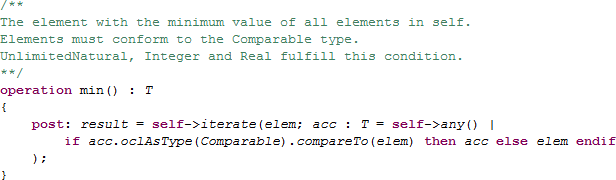
\includegraphics[width=5.75in]{Collection_min.png}
  \end{center}
  \caption{Collection::min.}
  \label{fig:Collection_min}
\end{figure}

An additional pre-condition, not yet supported by prototype tooling, should permit the implicit conformsTo Comparable within the postcondition to be expressed explicitly:

\verb|pre: self.oclType().elementType.oclIsKindOf(Comparable)|

\subsection{Summable}

A similar interface type may introduced to model the requirements of \verb|Collection::sum()| as shown in Figure~\ref{fig:Summable}.

\begin{figure}
  \begin{center}
    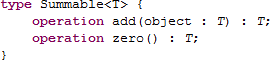
\includegraphics[width=2.75in]{Summable.png}
  \end{center}
  \caption{Summable.}
  \label{fig:Summable}
\end{figure}

If this interface type is realized by String as well as Real, then string splicing can be achieved by \verb|Sequence<String>::sum()|.

\section{Impact}

A number of new concepts have been introduced in this paper, but very few of them have any impact on OCL, merely on the ability to provide a modeled OCL specification.

From a user perspective, the main change is a recommendation to migrate towards \verb|< >| rather than \verb|( )| so that OCL has explicit UML-aligned templates rather than just template-like collections.

The clearer declarations and semantics for the library will require implementers to review their endeavors to interpret earlier specifications.

\begin{itemize}
\item Elimination of covariant overloading
\item Refactored Collection hierarchy
\item Comparable and Summable interfaces
\item oclAsSet
\end{itemize}

This will probably require some behavioral revision, which users can be protected from by providing an alternate OCL Standard Library with that a tool's traditional semantics.

Tools that offer OCL Standard Library customization will need to implement the library DSL and its associated interpretations of template and lambda types. Tools may choose to just re-use the standard UML-aligned OCL Standard Library Model, but this will still require support for the corollaries of UML alignment.

\begin{itemize}
\item Introduction of an Operation::precedence property
\item Introduction of an Operation::implementation property
\item Introduction of an Iteration class
\item Introduction of a LoopExp::referredIteration property 
\item Use of template type specializations
\item Use of template operation specializations
\item Use of template lambda type specializations
\end{itemize}


\section{Conclusions}

Elimination of typographical errors from the OCL specification was an original motivation for introduction of an OCL Standard Library model. But as we have shown the benefits are much greater; the model is readable, extensible, interchangeable and toolable.

We have described prototype Eclipse OCL tooling for a Domain Specific language for the OCL Standard Library model. This tooling enables the official model and extended models to be produced easily and reliably.

We have followed through some of the problems raised by attempts to model the library and revised the library content slightly and introduced additional concepts to support the model.

We have shown how modeled declarations can detect errors and provide definitive semantics for gaps in the current specification.

\nocite{*}
\bibliographystyle{eceasst}
\bibliography{ModelingOCLstdlib}

\end{document}
